\chapter{Governo digital no Judiciário}

O Brasil pós-democrático foi implementado como uma república  federativa, em concordância com \cite{cf88}, formada pela união indissolúvel dos Estados e Municípios e do Distrito Federal, constitui-se em Estado Democrático de Direito, cujos Poderes são o Executivo, Legislativo e Judiciário.

Haja vista o foco deste trabalho é o Poder Judiciário, o Poder Judiciáiro é composto, segundo \cite{cf88}, no art. 92 da CRFB:

\begin{itemize}
    \item Supremo Tribunal Federal.
    \item Conselho Nacional de Justiça.
    \item Superior Tribunal de Justiça.
    \item Tribunal Superior do Trabalho.
    \item Tribunais Regionais Federais e Juízes Federais.
    \item Tribunais e Juízes do Trabalho.
    \item Tribunais e Juízes Eleitorais.
    \item Tribunais e Juízes Militares.
    \item  Tribunais e Juízes dos Estados e do Distrito Federal e Territórios.
\end{itemize}

\cite{cf88} concedeu ao Poder Judiciário autonomia administrativa e financeira. A importância da autonomia para o Poder Judiciário se confirma ao analisar as figuras \ref{fig:jus_constraints_on_gov} e \ref{fig:judicial-corruption-score}.

\begin{figure}[H]
    \centering
    \caption{Índice de controle judicial sobre o Poder Executivo}
    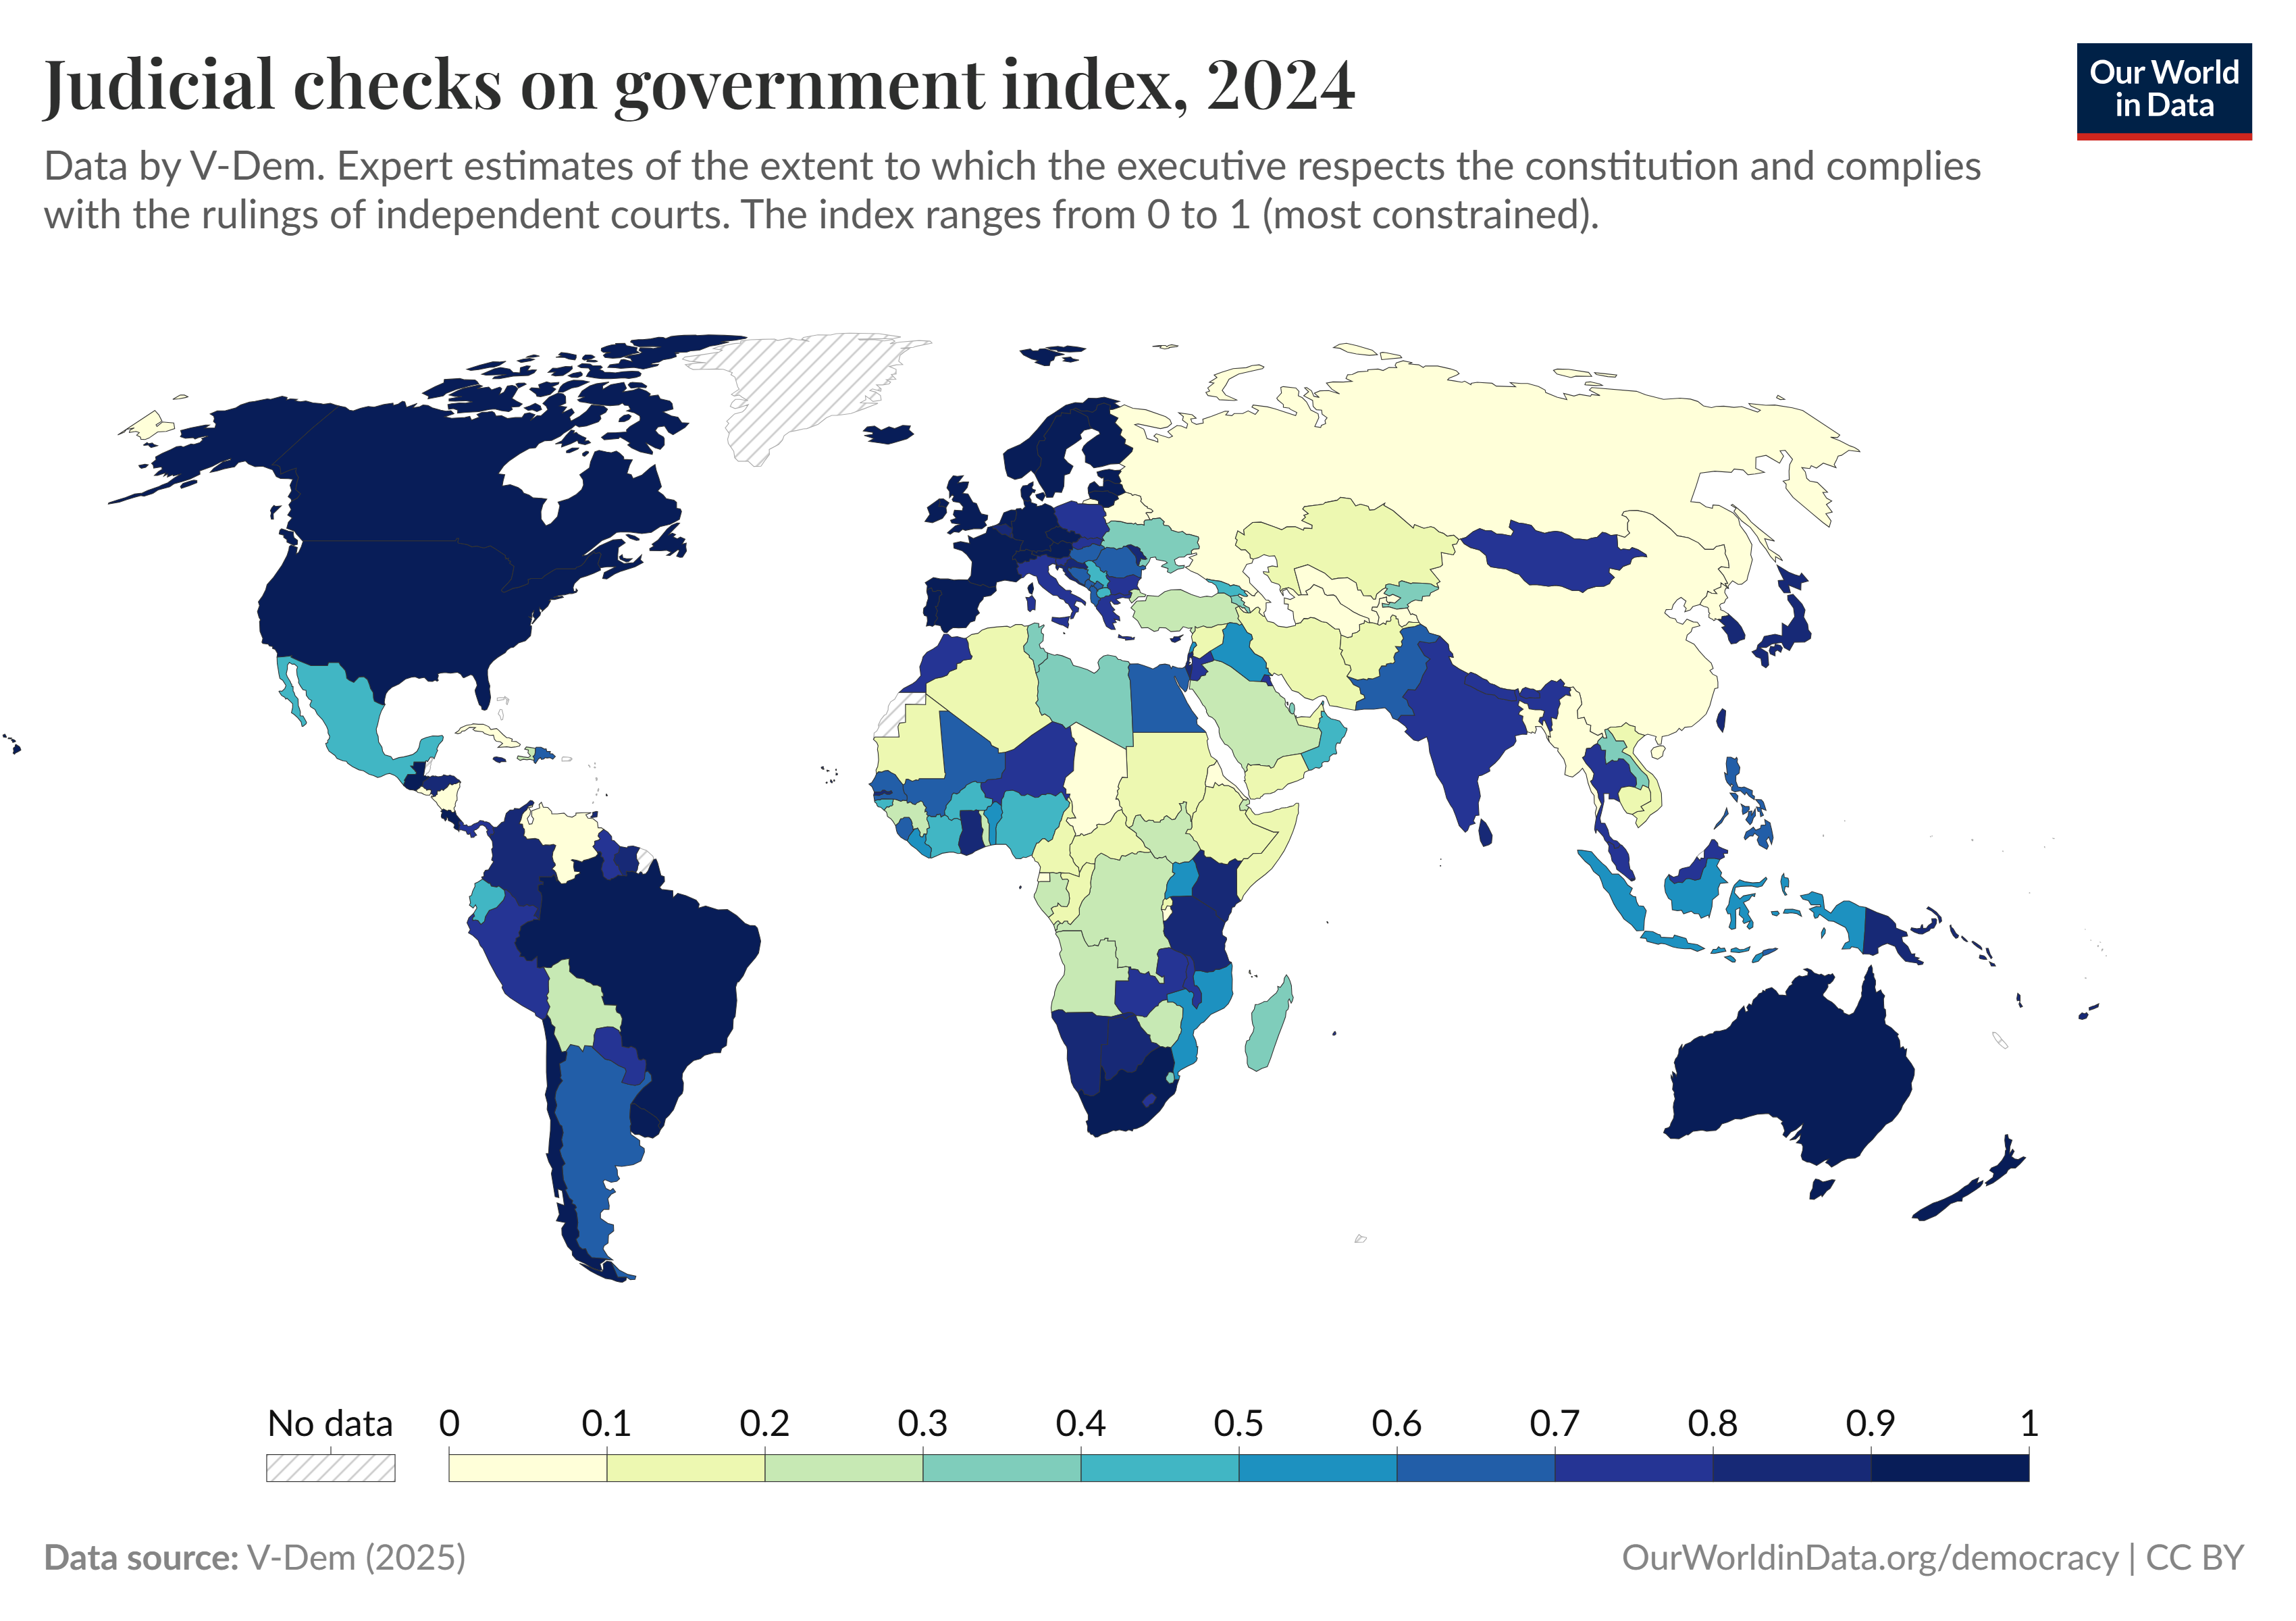
\includegraphics[width=1\linewidth]{figuras/judicial-constraints-on-the-executive-index.png}
    \label{fig:jus_constraints_on_gov}
    \footnotesize{Fonte: \cite{jus_constraints_on_gov}.}
\end{figure}

No tocante a figura \ref{fig:jus_constraints_on_gov}, nota-se como a democracia melhorou os índices do Brasil. Em 2024, o Brasil quase atingiu o valor máximo - 0,96 - enquanto a média mundial foi 0,664. Apenas 31 países de 193 - equivalente a 16\% do total - alcançaram uma pontuação de, no mínimo, 0,9 de 1,0 até o máximo.

A figura \ref{fig:quartis_controle_jus_sobre_gov} contém o diagrama da caixa: índice de controle judicial sobre o Poder Executivo.

\begin{figure}[H]
    \centering
    \caption{Diagrama da caixa: índice de controle judicial sobre o Poder Executivo}
    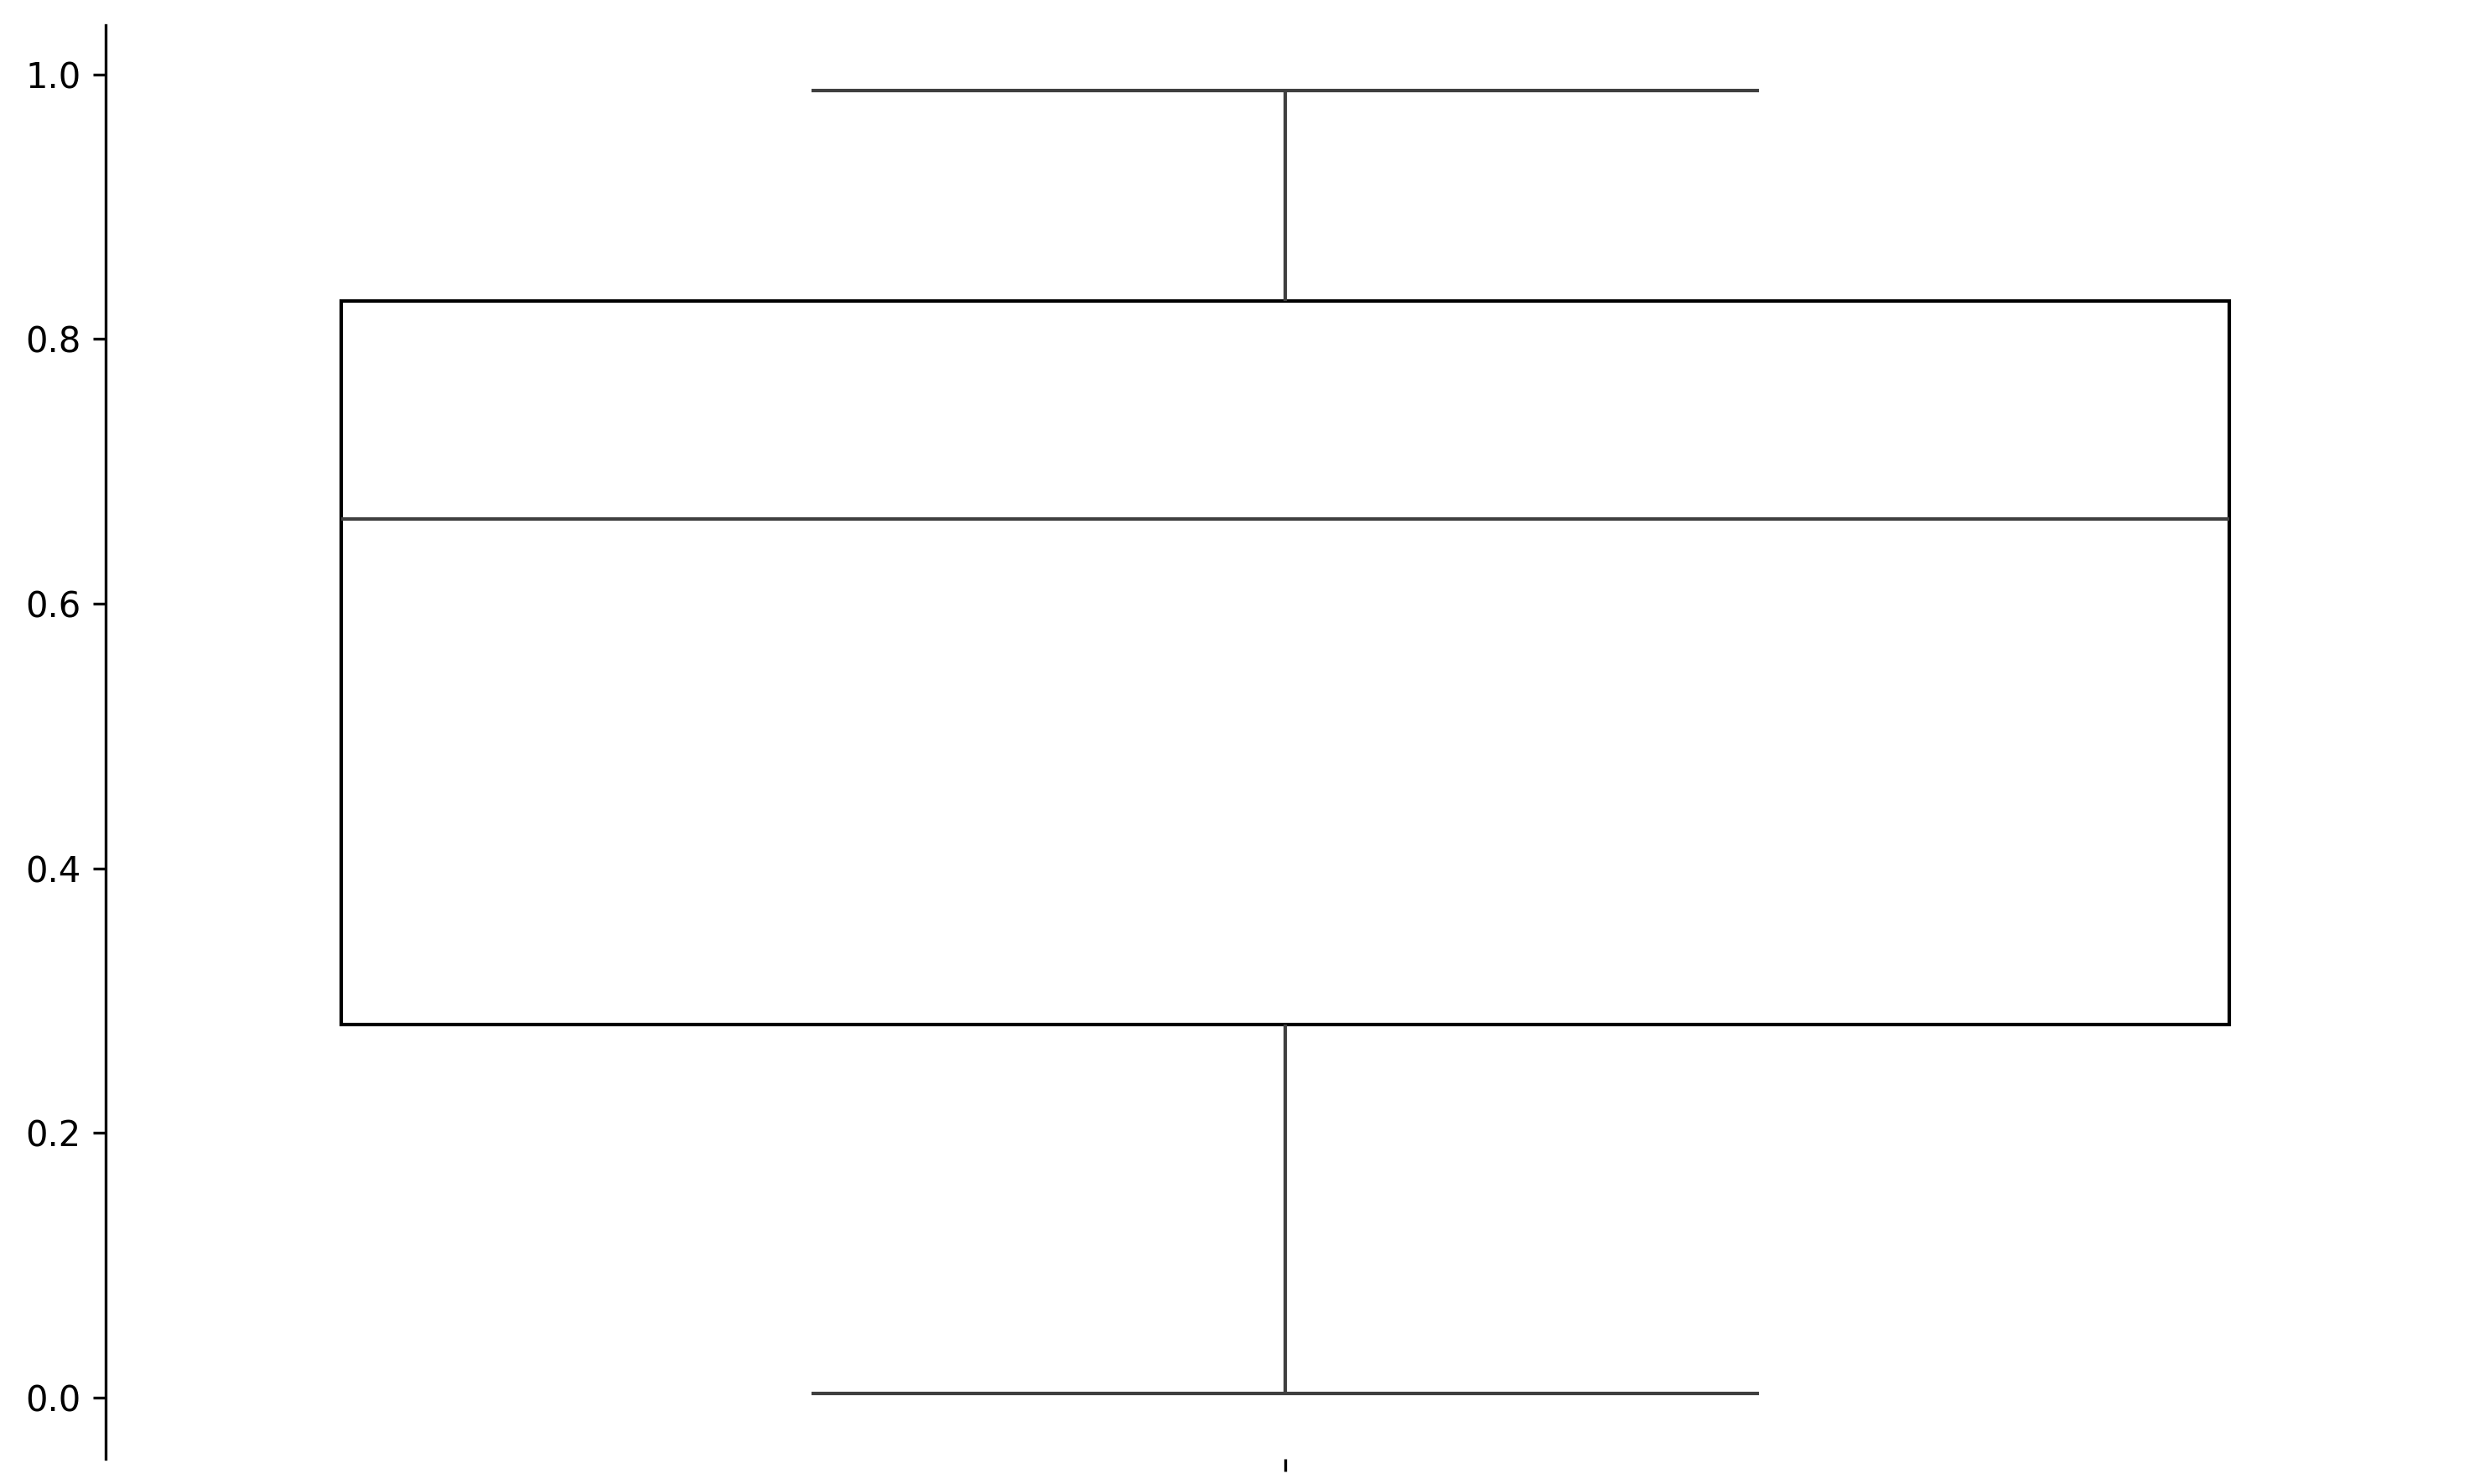
\includegraphics[width=1\linewidth]{figuras/quartis_controle_jus_sobre_gov.png}
    \label{fig:quartis_controle_jus_sobre_gov}
    \footnotesize{Fonte: elaboração própia baseada em \cite{jus_constraints_on_gov}.}
\end{figure}

A figura \ref{fig:quartis_controle_jus_sobre_gov}, que mostra a distribuição do índice de controle judicial sobre o Poder Executivo, ilustra que no ano de 2024 teve um valor mínimo de 0,003 e um máximo de 0,988. A média dos dados foi de 0,664. Além disso, 25\% dos valores ficaram abaixo de 0,282 (1º quartil), enquanto 75\% dos valores foram inferiores a 0,829 (3º quartil).

A figura \ref{fig:judicial-corruption-score} mostra como o Brasil melhorou o aspecto da corrupção judiciária. 

\begin{figure}[H]
    \centering
    \caption{Pontuação de corrupção judicial}
    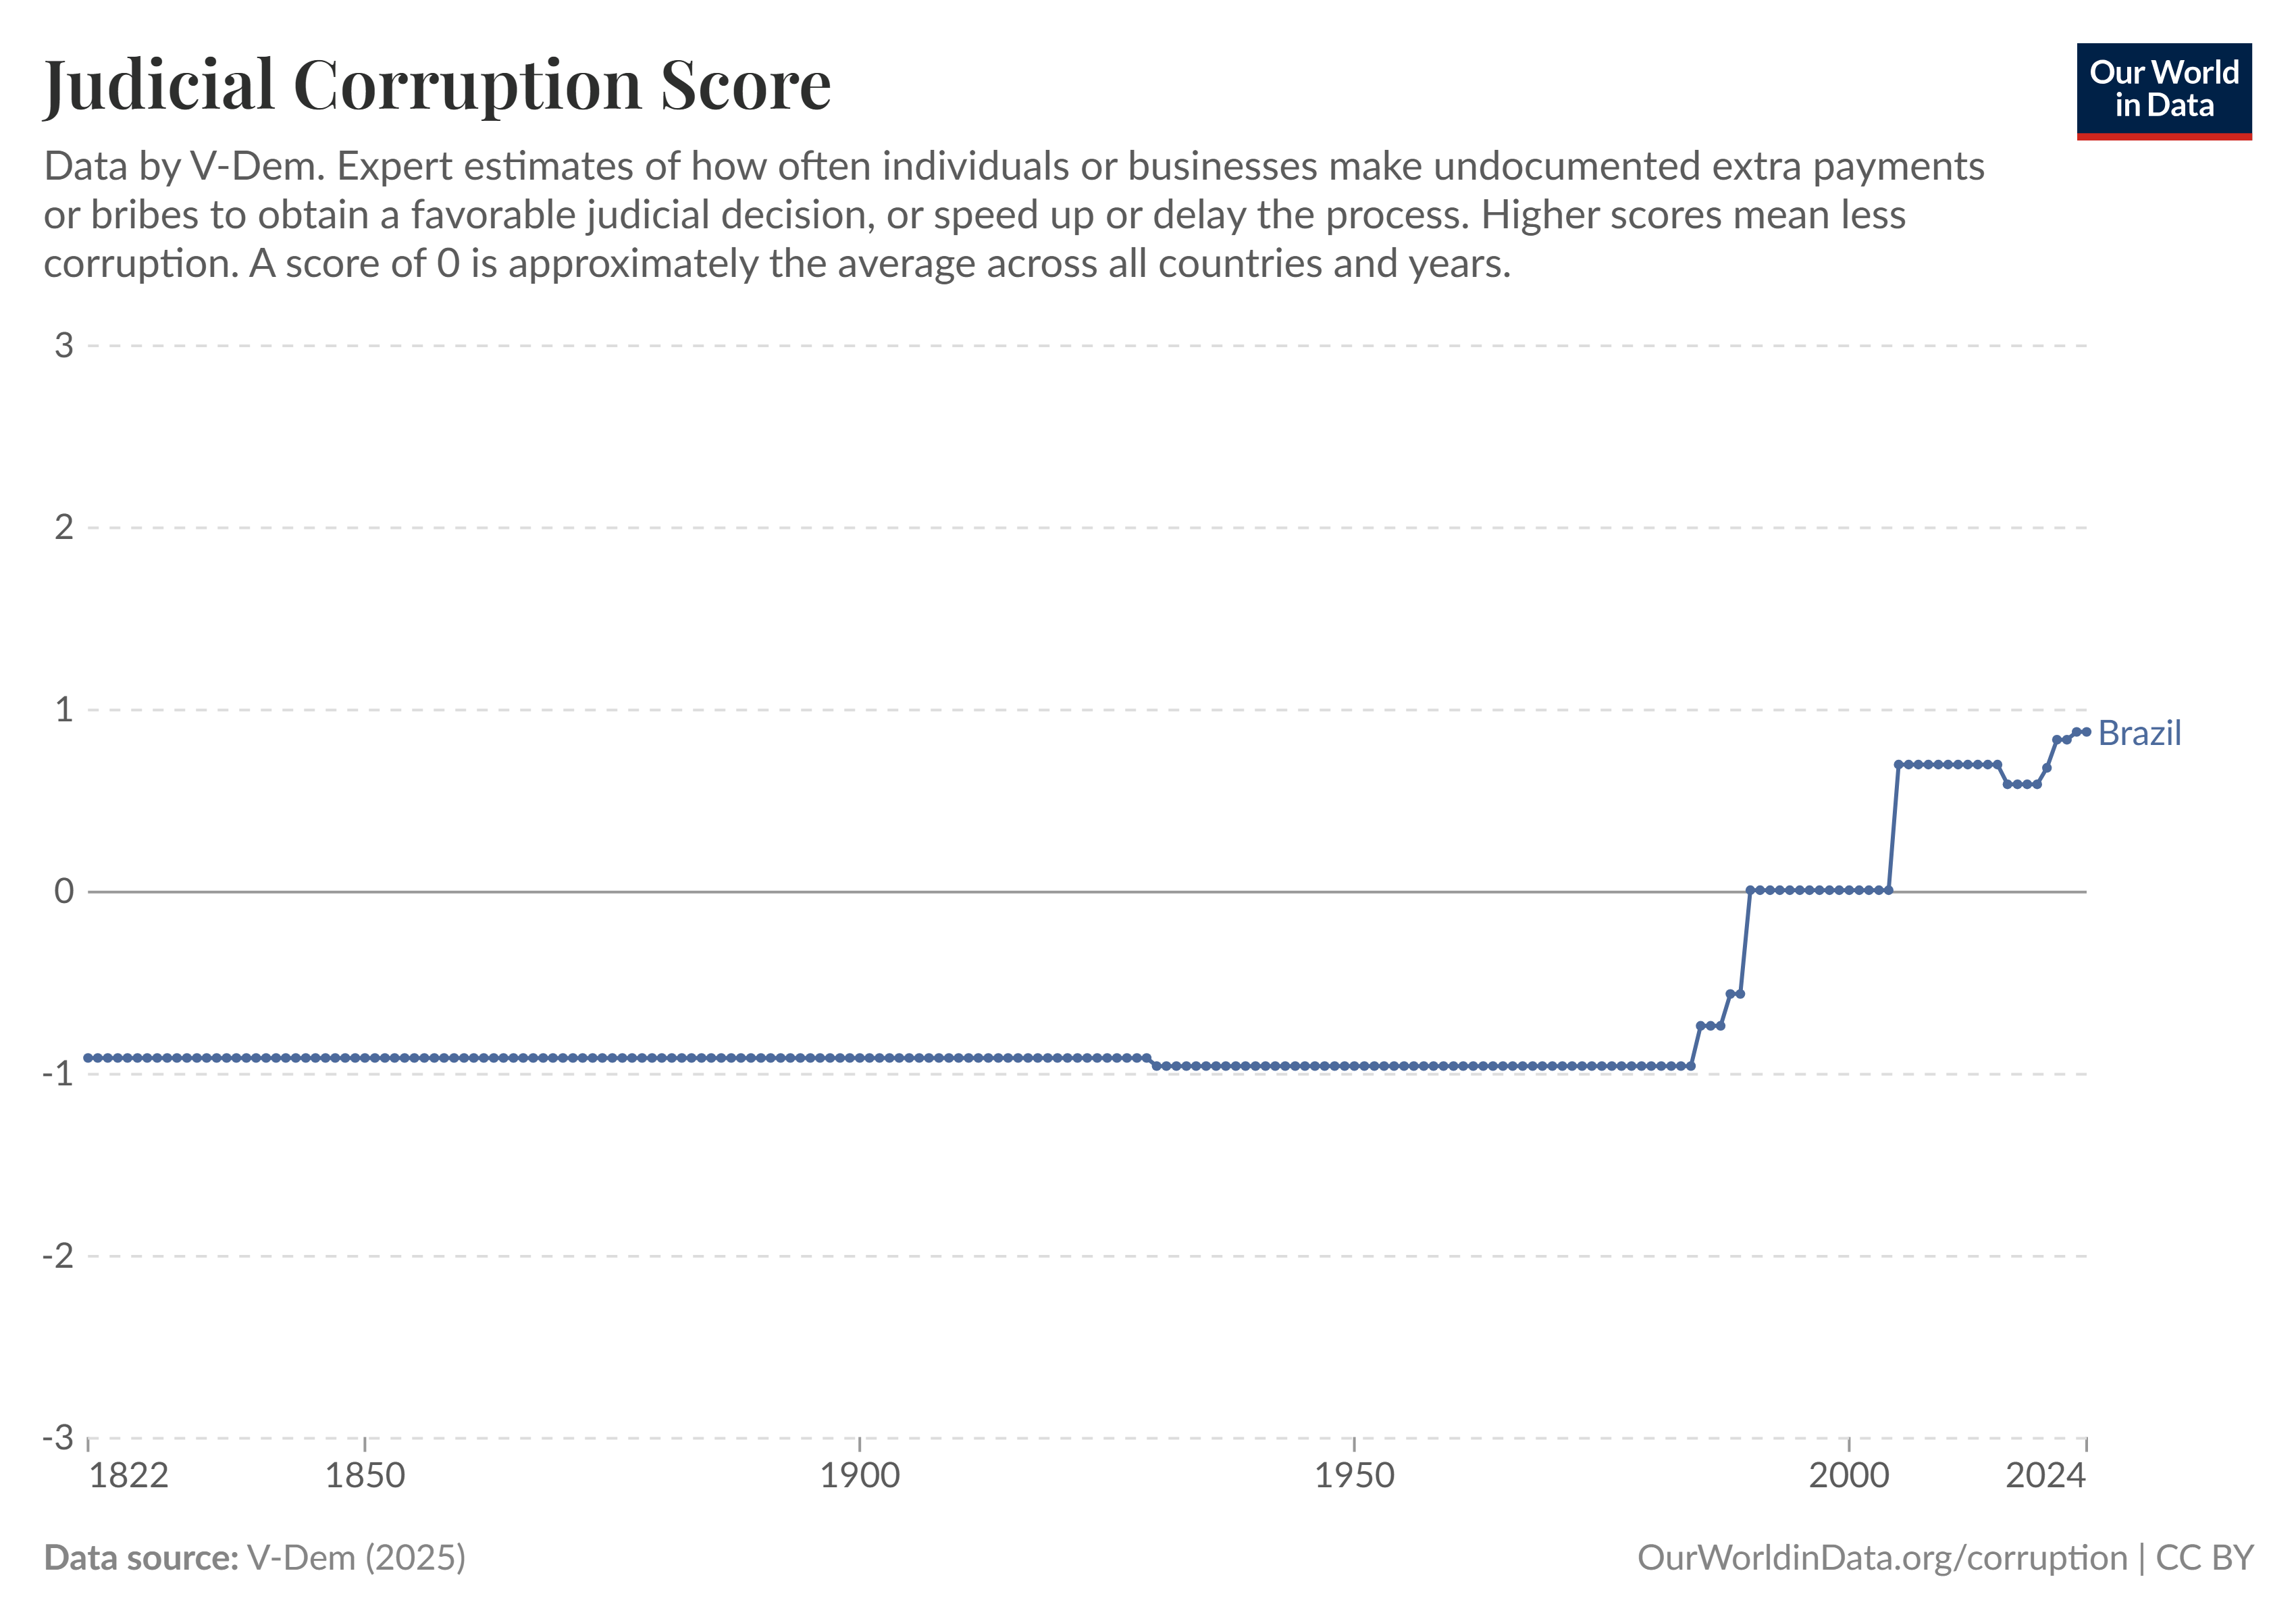
\includegraphics[width=1\linewidth]{figuras/judicial-corruption-score.png}
    \label{fig:judicial-corruption-score}
    \footnotesize{Fonte: \cite{judicial-corruption-score}.}
\end{figure}

Durante décadas, o Brasil ficou na faixa -1, alcançando 0 até 0,88. A atual pontuação do Brasil não está entre as melhores, pois ainda há as pontuações 2 e 3. No entanto, como a média mundial foi 0,249, o Brasil está acima da média mundial, porém o país foi superado por 66 países, cujas pontuações superaram 0,88. A quantidade de países que atingiu, no mínimo, 1 foi 29,84\%; no tocante a pontuação 2, foi 12\%; e por fim, 3 foi 3\% e nenhum atingiu 4 (valor máximo).

De maneira complementar, a figura \ref{fig:quartis_corrupcao_judiciaria} contém o diagrama de caixa da pontuação de corrupção judicial.

\begin{figure}[H]
    \centering
    \caption{Diagrama da caixa: corrupção judicária}
    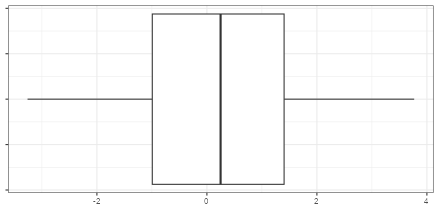
\includegraphics[width=1\linewidth]{figuras/quartis_corrupcao_judiciaria.png}
    \label{fig:quartis_corrupcao_judiciaria}
    \footnotesize{Fonte: elaboração própria baseada em \cite{judicial-corruption-score}.}
\end{figure}

A figura \ref{fig:quartis_corrupcao_judiciaria}, que mostra a distribuição do índice de corrupção judiciária, ilustra que no ano de 2024 teve um valor mínimo de -3,2610 e um máximo de 3,7690. A média dos dados foi de 0,2490. Além disso, 25\% dos valores ficaram abaixo de -0,9930 (1º quartil), enquanto 75\% dos valores foram inferiores a 1,4035 (3º quartil).

O Brasil está em posição privilegiada, pois, se apenas 25\% dos 193 países alcançaram uma pontuação superior e metade alcançou menos que a média mundial, isso é um indicativo de que autocracias são prevalentes. \cite{nord2025democracy} informa que o Brasil, juntamente com o Equador, Lesoto e a Polônia, pararam e reverteram processos de autocratização antes da disrupção da democracia, exibindo resiliência a rupturas autocráticas.

Outros dados que reforçam a importância da democracia no Brasil foram apresentados por \cite{nord2025democracy} no relatório Democracy Report 2025 da V-Dem relativo ao ano de 2024 na lista abaixo:

\begin{itemize}
    \item Democracias liberais representam menos de 12\% da população mundial, ou seja, menos de 900 milhões de pessoas.
    \item Democracias eleitorais representam 17\% da população mundial.
    \item 40\%  da população mundial - 3,1 bilhões de pessoas - vive em países que estão em processo de autocratização.
    \item Há mais autocracias do que democracias no mundo: 91 contra 88. Em 2023, era o contrário.
    \item O mundo tem apenas 29 liberais, o que torna o regime o mesmo comum.
    \item 72\% das pessoas no mundo vivem em autocracias, percentual mais alto desde 1978.
\end{itemize}

As informações alarmantes apresentadas por \cite{nord2025democracy} expõem o quão benéfica tem sido a democracia para o Brasil desde a redemocratização. Embora o Brasil ainda apresente desafios, o país está em processo de melhoria institucional. Um exemplo disso é o fato do Brasil ter tido a capacidade de reverter uma tentativa de autocratização enquanto 40\%  da população mundial vive em países que estão em processo de autocratização.

Como consequência da argumentação anterior, \cite{pires2021paradoxo} corrobora a independência do Poder Judiciário. Para o autor, o Poder Judiciário obteve níveis elevados de independência com a CRFB de 1988, que em um esforço para fortalecer a independência individual dos juízes, os termos e condições de mandato foram significativamente aprimorados.  Bem como, a CRFB também fortaleceu a independência funcional do judiciário como instituição de governança, isolando-o do sistema político mais amplo.

Como resultado da independência proporcionada pela CRFB, \cite{pires2021paradoxo} cita que os tribunais receberam controle total sobre seus assuntos administrativos, pessoais e disciplinares, de modo que o Poder Judiciário obteve controle quase total sobre seu orçamento.

Como forma de evitar a ingerência do Poder Executivo, \cite{pires2021paradoxo} argumenta que a CRFB estabeleceu o STF é o responsável pela elaboração do orçamento anual da Justiça Federal e pelo encaminhamento direto ao Congresso Nacional. Assim, limitou-se o poder do Governo Federal sob o Poder Judiciário, evitando a constrição do orçamento do Poder Judiciário, por quaisquer motivos do Poder Executivo, tornando factível a independência do Poder judicante.

Outro autor destacou a importância da independência do Poder Judiciário foi \cite{akutsu2012dimensoes}. Para ele, a importância de um Poder Judiciário independente dos Poderes Executivo e Legislativo decorre da necessidade de salvaguarda da liberdade individual dos cidadãos, que podem recorrer ao Judiciário contra abusos de autoridades de quaisquer dos três poderes. 

Para \cite{akutsu2012dimensoes}, a independência do Poder Judiciário não deve constituir óbice do cumprimento dos princípios e às normas da CRFB pelos juízes. Além de poder serem responsabilizados perante os cidadãos. 

Complementarmente, para \cite{akutsu2012dimensoes} no caso da premissa da independência dos juízes e tribunais não se concretize, o desempenho do Poder Judiciário pode ser afetado, uma vez que os juízes enfrentariam óbices para  proferir sentenças que desagradassem pessoas afetadas por suas decisões.

Como fortalecedor da independência do Poder Judiciário, e como demonstração constitucional de sua importância para o Brasil, em 2004 o Congresso Nacional aprovou a EC nº 45, de 2004. \cite{ec45_2004} criou o CNJ, as Súmulas Vinculantes do STF, extinguiu os Tribunais de Alçada e determinou sua incorporação aos Tribunais de Justiça, além das outras medidas estabelecidas.

No contexto da mudança legislativa promovida pela  EC nº 45, de 2004, a criação do Conselho Nacional de Justiça (CNJ), através da publicação da referida Emenda à Constituição, foi precedida e sucedida de diversas celeumas relaciona das à sua natureza, constitucionalidade, legitimidade e efetividade.

Para \cite{silva2013transparencia}, a criação do CNJ, promovida pela publicação da EC nº 45, de 2004, foi precedida e sucedida de diversas celeumas relaciona das à sua natureza, constitucionalidade, legitimidade e efetividade.  

Ao CNJ, segundo \cite{silva2013transparencia}, foram concedidos importantes poderes para que o órgão, respondendo do constituinte derivado, respondendo pelo controle da atuação administrativa e financeira do Poder Judiciário. São competências do CNJ, conforme \cite{cf88}, no art. 103-B, §4º, \textit{ipsi litteris}:

"§ 4º Compete ao Conselho o controle da atuação administrativa e financeira do Poder Judiciário e do cumprimento dos deveres funcionais dos juízes, cabendo-lhe, além de outras atribuições que lhe forem conferidas pelo Estatuto da Magistratura: I - zelar pela autonomia do Poder Judiciário e pelo cumprimento do Estatuto da Magistratura, podendo expedir atos regulamentares, no âmbito de sua competência, ou recomendar providências; II - zelar pela observância do art. 37 e apreciar, de ofício ou mediante provocação, a legalidade dos atos administrativos praticados por membros ou órgãos do Poder Judiciário, podendo desconstituí-los, revê-los ou fixar prazo para que se adotem as providências necessárias ao exato cumprimento da lei, sem prejuízo da competência do Tribunal de Contas da União; III - receber e conhecer das reclamações contra membros ou órgãos do Poder Judiciário, inclusive contra seus serviços auxiliares, serventias e órgãos prestadores de serviços notariais e de registro que atuem por delegação do poder público ou oficializados, sem prejuízo da competência disciplinar e correicional dos tribunais, podendo avocar processos disciplinares em curso, determinar a remoção ou à disponibilidade e aplicar outras sanções administrativas, assegurada ampla defesa; IV representar ao Ministério Público, no caso de crime contra a administração pública ou de abuso de autoridade; V rever, de ofício ou mediante provocação, os processos disciplinares de juízes e membros de tribunais julgados há menos de um ano; VI elaborar semestralmente relatório estatístico sobre processos e sentenças prolatadas, por unidade da Federação, nos diferentes órgãos do Poder Judiciário;    VII elaborar relatório anual, propondo as providências que julgar necessárias, sobre a situação do Poder Judiciário no País e as atividades do Conselho, o qual deve integrar mensagem do Presidente do Supremo Tribunal Federal a ser remetida ao Congresso Nacional, por ocasião da abertura da sessão legislativa."          

As competências presentes no art. 103-B, §4º da CRFB empoderam o CNJ como ordenador do Poder Judiciário . E como tal, o órgão tem modernizado o Poder Judiciário via seus atos administrativos. Para realizar suas ações de modernização, e como o CNJ integra a Administração Direta, suas ações, quaisquer que sejam, devem estar no rol das ações autorizadas nas leis orçamentárias da União aprovadas pelo Congresso Nacional, nos termos da CRFB.

A figura \ref{fig:diagrama_linha_orçamento_justiça_2010_2025} mostra como o orçamento do Poder Judiciário da União evoluiu de 2010 até 2025.

\begin{figure}[H]
	\centering
	\caption{Evolução do orçamento do Poder Judiciário da União (2010-2025)}
	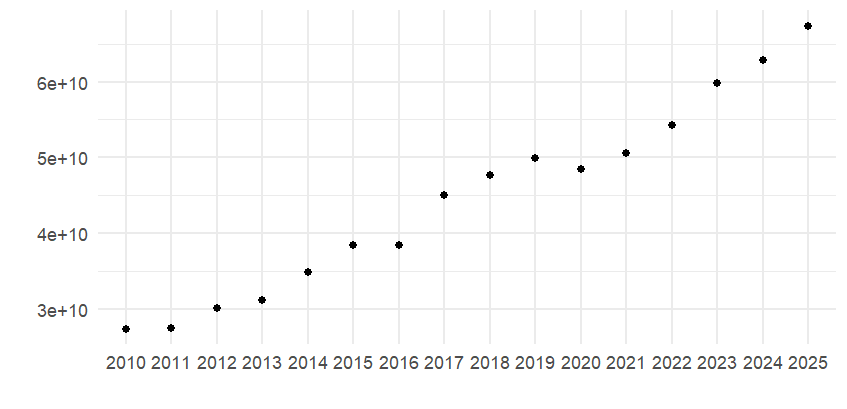
\includegraphics[width=1\linewidth]{figuras/diagrama_linha_orçamento_justiça_2010_2025}
	\label{fig:diagrama_linha_orçamento_justiça_2010_2025}
	\footnotesize{Fonte: elaboração própria baseada em \cite{}.}
\end{figure}

Da figura \ref{fig:diagrama_linha_orçamento_justiça_2010_2025}, nota-se que há uma tendência de crescimento, com poucos pontos de queda em relação ao ano anterior.

Assim, as figuras \ref{fig:diagrama_barras_orçamento_orgaos_justiça_2010_2025} e \ref{fig:diagrama_barras_orçamento_cnj_2010_2025} mostram a participação percentual individual de cada órgão do Poder Judiciário da União e a evolução do orçamento do CNJ nas LOA da União de 2010 até 2025. Optou-se por não incluir os anos anteriores a 2010, pois, de 2010 em diante, o CNJ passou a aparecer de forma individualizada no orçamento da União.

\begin{figure}[H]
	\centering
	\caption{Participação percentual dos órgãos do Poder Judiciário relativa ao orçamento total do Poder Judiciário} 
	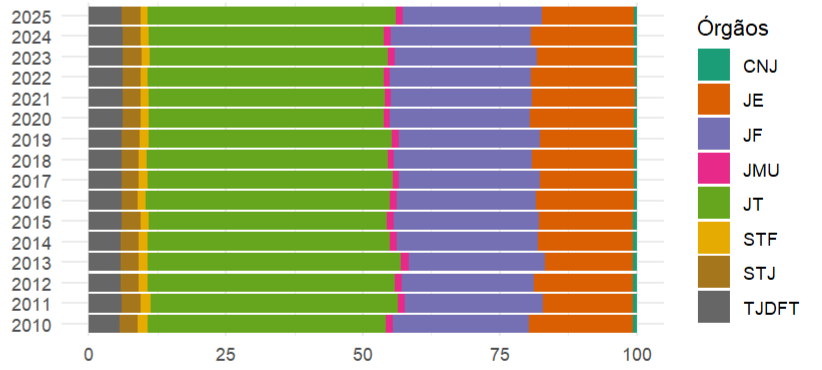
\includegraphics[width=1\linewidth]{figuras/diagrama_barras_orçamento_orgaos_justiça_2010_2025}
	\label{fig:diagrama_barras_orçamento_orgaos_justiça_2010_2025}
	\footnotesize{Fonte: elaboração própria baseada em \cite{}.}
\end{figure}

Dos órgãos do Poder Judiciário da União, a Justiça do Trabalho é a mais dispendiosa, seguidas da Justiça Federal e Eleitoral. Dos órgãos menos dispendiosos, estão o TJDFT, STJ, STF, JMU, e o CNJ. Como o CNJ tem o menor orçamento dentro do Poder Judiciário da União, ele praticamente foi invisibilizado pelo demais órgãos na figura \ref{fig:diagrama_barras_orçamento_orgaos_justiça_2010_2025}.

\begin{figure}[H]
	\centering
	\caption{Orçamento anual do CNJ (2010-2025)} 
	\includegraphics[width=1\linewidth]{figuras/diagrama_barras_orçamento_cnj_2010_2025}
	\label{fig:diagrama_barras_orçamento_cnj_2010_2025}
	\footnotesize{Fonte: elaboração própria baseada em \cite{}.}
\end{figure}


%\section{Orçamento do Poder Judiciário}

%\section{Orçamento-programa da digitalização do Poder Juciário}

%Modernização do poder judiciário

%\section{Políticas públicas de governo digital no Judiciário}

%Creta

%Processo judicial eletrônico

%\Plataforma Digital do Poder Judiciário Brasileiro

%Justiça 4.0

%Justiça Aberta}

%DataJud

%https://www.cnj.jus.br/pesquisas-judiciarias/paineis-cnj/